\section{Rig Analysis}

\begin{figure}[ht]
  \centering
  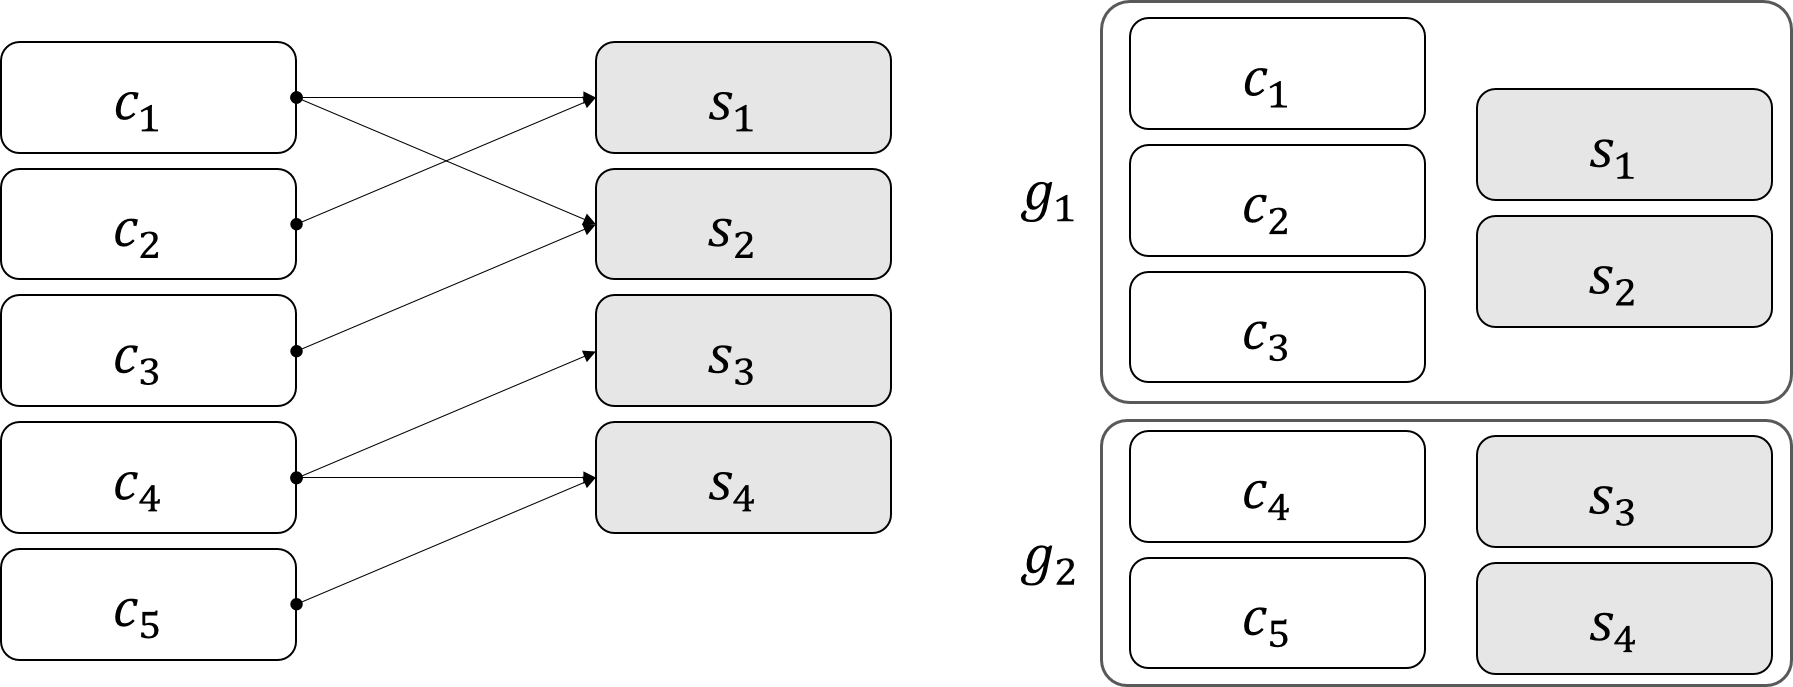
\includegraphics[width=0.95\linewidth]{images/correlationMap}
  \caption{(a)  Correlation map between rig space and skeleton space. (b) Body part grouping based on the correlation map}
  \label{fig:correlationMap}
\end{figure}
We formulate our inverse mapping as an optimization problem on the Lie algebra space. However, simultaneous optimization of all the parameters in the skeleton space and the rig space would not be efficient, because some of the rig parameters do not have any influence on some of the skeletons. Unfortunately, we do not have any prior information to identify these relationship. Therefore, we perform analysis with the following strategies:
\begin{itemize}
	\item Define the correlation map between the rig space parameter and the skeleton segment
	\item Divide the rig into several groups for which the rig operations are mutually independent 
\end{itemize}
After the rig analysis, we perform the optimization separately for each rig group. The rig analysis process is summarized in Algorithm 1.
\begin{algorithm}[ht]
    \caption{Rig Analysis}
    \SetKwInOut{Input}{Input}
    \SetKwInOut{Output}{Output}
    
    \Input{
	    Rig space parameters $\mathbf{c} = \left\{c_1, ..., c_m\right\}$,\newline
	    Individual skeletal segment parameters $\mathbf{s} = \left\{s_1, ..., s_k\right\}$
	    }
    \Output{
    Body part groups $G = \left\{g_1,g_2, ..., g_l\right\}$,\newline
    %Each group $g_i$ contains a set of corresponding rig parameters, skeleton parameters, \newline
    %Rig operations of $g_i$ in $G$ are mutually independent
    }
    $G \leftarrow \left\{g_1, ..., g_m\right\}$\;
    \For{each $c_i$ in $\mathbf{c}$}{
    		$g_i \leftarrow c_i$\;
    		$\check{\mathbf{c}}_i \leftarrow r \times randomSampling(c_i)$\;
    		$\check{\mathbf{p}}_\mathbf{s} \leftarrow poseMeasure(\check{\mathbf{c}}_i)$\;
    		
    		\For{each $s_j$ in $\mathbf{s}$}{
    			$\rho_{i,j} \leftarrow multipleCorrelation(\check{\mathbf{c}}_i, \check{\mathbf{p}}_{s_j})$\;
    			\If{$\rho_{i,j} \geq 0.5$}{
    				$g_i \leftarrow g_i \cup s_j$\;
    			}
    		}
    }
    \For{$\left\{g_i, g_j\right\}$ in $G$}{
	    \If{$\left\{g_i, g_j\right\}$ has same element}{
	    		merge $g_i$ and $g_j$\;
	    }
    }
   
   
    
%    create group $\hat{G} = \{\hat{g}_1, \dots, \hat{g}_m\}$\;
%    $\{\check{\mathbf{c}},\check{\mathbf{S}}\} \leftarrow r$ times of random value sampling per each $c$ in $C$\;
%	%\tcc*[h]{Random Value Sampling Process}\\
%	\For{ $c_i$ in $\mathbf{c}$, $s_j$ in $\mathbf{s}$ }{
%		%$k$ times of random value sampling for rig space parameter $c_i$ (range: $c_{min}<c_i<c_{max}$)\;
%		$\check{\mathbf{c}}_i \leftarrow \left\{ \check{c}^1_i, \dots, \check{c}^r_i \right\}$\;
%		$\check{\mathbf{s}}^j_{i} \leftarrow \left\{ \check{s}^{i,j}_0, \dots, \check{s}^{i,j}_k \right\}$\;
%		$\rho_{i,j} \leftarrow MultipleCorrelationCoefficient(\check{\mathbf{c}}_i, \check{\mathbf{s}}_i^j)$\;
%		%compute multiple correlation coefficient $\rho_{i,j}$ between $c_i$ and $s_j$ with sampled data list\;
%		\If {$\rho_{i,j} > 0.5$}{
%	    		union $g_i$ and $\{c_i, s_j\}$\;
%	    	}
%	}
%	%\tcc*[h]{Grouping Process}\\
%	\Repeat{no more groups have same element}{
%		\If{$g_i$ and $g_j$ have same element}{
%			union $g_i$ and $g_j$\;
%		}
%	}
	%\Return{$g = {g_1, ..., g_l}$}\;
\end{algorithm}
For a character composed of rig parameters $\mathbf{c}=\left\{ c_1, \dots, c_m \right\}$ and skeleton segments $\mathbf{s}=\left\{ s_1, \dots, s_k \right\}$,
we first define a \textit{correlation map} between $\mathbf{c}$ and $\mathbf{s}$.
Note that we only exploit relative transformation $A_{s_p,s_i}$ in the local coordinate system of $s_i$ about the parent skeletal segment $s_p$ during the rig analysis stage, to find \textit{direct} correlation between $c_j$ and $s_i$.
To construct a correspondence map without any prior information, we perform $r$ times of random value sampling per each $c_i$ in $\mathbf{c}$, and then measure the transformation changes of $\mathbf{s}$.
Then, we calculate multiple correlation coefficient $\rho_{i,j}$ between $c_i$ and $s_j$ that are sampled and measured data, respectively.
This represents correlation between $c_{i}$ and $s_{j}$  with a scalar value of range 0 to 1. Although the interpretation for the value of $\rho_{i,j}$ may depend on the context and purposes, we assume that $\rho_{i,j} < 0.5$ means that the two variables have no strong linear relationship\cite{mark2001practical}.

%Then, for each sample set for $c_i$, we calculate multiple correlation coefficient $\rho_{i,j}$ between $\check{\mathbf{c}}_i$ and $s_j$ using measured skeletal pose.
%$\check{\mathbf{c}}_i = \left \{ \check{c}^1_{i}, \check{c}^2_{i}, \dots, \check{c}^r_{i} \right \}$
%The sampled and measured data per each $c_i$ are represented as $\check{\mathbf{c}}_i = \left \{ \check{c}^1_{i}, \check{c}^2_{i}, \dots, \check{c}^r_{i} \right \}$.
%\def \cp {\check{\mathbf{p}}}
%\def \cc {\check{\mathbf{c}}}
%\begin{equation}
%	\begin{split}
%		\cc{}_i &= \left \{ \check{c}^1_{i}, \check{c}^2_{i}, \dots, \check{c}^r_{i} \right \}, \\
%		%\check{\mathbf{c}} &= \left \{ \check{c}^1_{1}, \check{c}^2_{1}, \dots, \check{c}^r_{m-1}, \check{c}^r_{m} \right \}, \\
%		\cp{}_i &= \left \{ \cp{}(\check{c}^1_i) \ldots \cp{}_i(\check{c}^r_i) \right \},
%	\end{split}
%\end{equation}
%
%Here, $\check{\mathbf{c}}_i$ is set of $r$ sampled rig parameters where $\check{c}^j_{i}$ denotes the $j$-th random value for $c_i$,
%and $\check{\mathbf{p}}_i$ is set of $r$ measured pose where $f(\check{c}^1_{i})$ denotes skeleton segments $\mathbf{s}$ given $\check{c}^j_{i}$.
%%$\check{\mathbf{s}}^j_{i} = \left\{ \check{s}^{i,j}_0, \dots,\check{s}^{i,j}_k \right\}$
%%$D_c$ and $D_s$ are the generated data lists by sampling.
%Next, we compute multiple correlation coefficient $\rho$ between
%$\check{\mathbf{c}}_i = \left\{ \check{c}^1_i, \dots, \check{c}^r_i \right\}$ which represents set of samples for $c_i$, and $\mathbf{s}_i = \left\{ \check{\mathbf{s}}_i^1 \ldots \check{\mathbf{s}}_i^r \right\}$.
%This returns 
%%$\check{\mathbf{s}}^j_i(n) = \left\{ \check{s}^{i,1}_j, \dots, \check{s}^{i,r}_j \right\}$.
%%$\check{c}_{i} \in r \times \mathbb{R}^1$ and $\check{s}_{j} \in r \times \mathbb{R}^6$ 
%This represents correlation between $c_{i}$ and $s_{j}$  with a scalar value of range 0 to 1. Although the interpretation for the value of $\rho_{i,j}$ may depend on the context and purposes, we assume that $\rho_{i,j} < 0.5$ means two variables have no strong linear relationship\cite{mark2001practical}.
%%In this way, we define the correlation map between $c$ and $s$ based on $\rho$.
%Figure~\ref{fig:correlationMap} (left) shows an example of the correlation map.
%If a $s_i$ is transformed when $c_j$ is modified, then the two parameters are connected.
%

The second goal of the rig analysis is to divide the rig into mutually independent groups.
We generate a set $\left\{g_1, g_2, \dots, g_m\right\}$ as the same size as $\mathbf{c}$ where each element of $g_i$ consists of $c_i$ and a set of skeletal segments $s_*$ whose $\rho_{i,*}$ is bigger than 0.5. Next, if any $\left\{g_i, g_j\right\}$ have at least one element in common, the two groups are merged. We merge repeatedly until there is no intersection among the 2 groups. The result is mutually independent rig groups $G$:
\begin{equation}
	G = \left \{ {g_{1}, g_{2}, ..., g_{l}} \right \},
\end{equation}
\begin{figure}[ht]
  \centering
  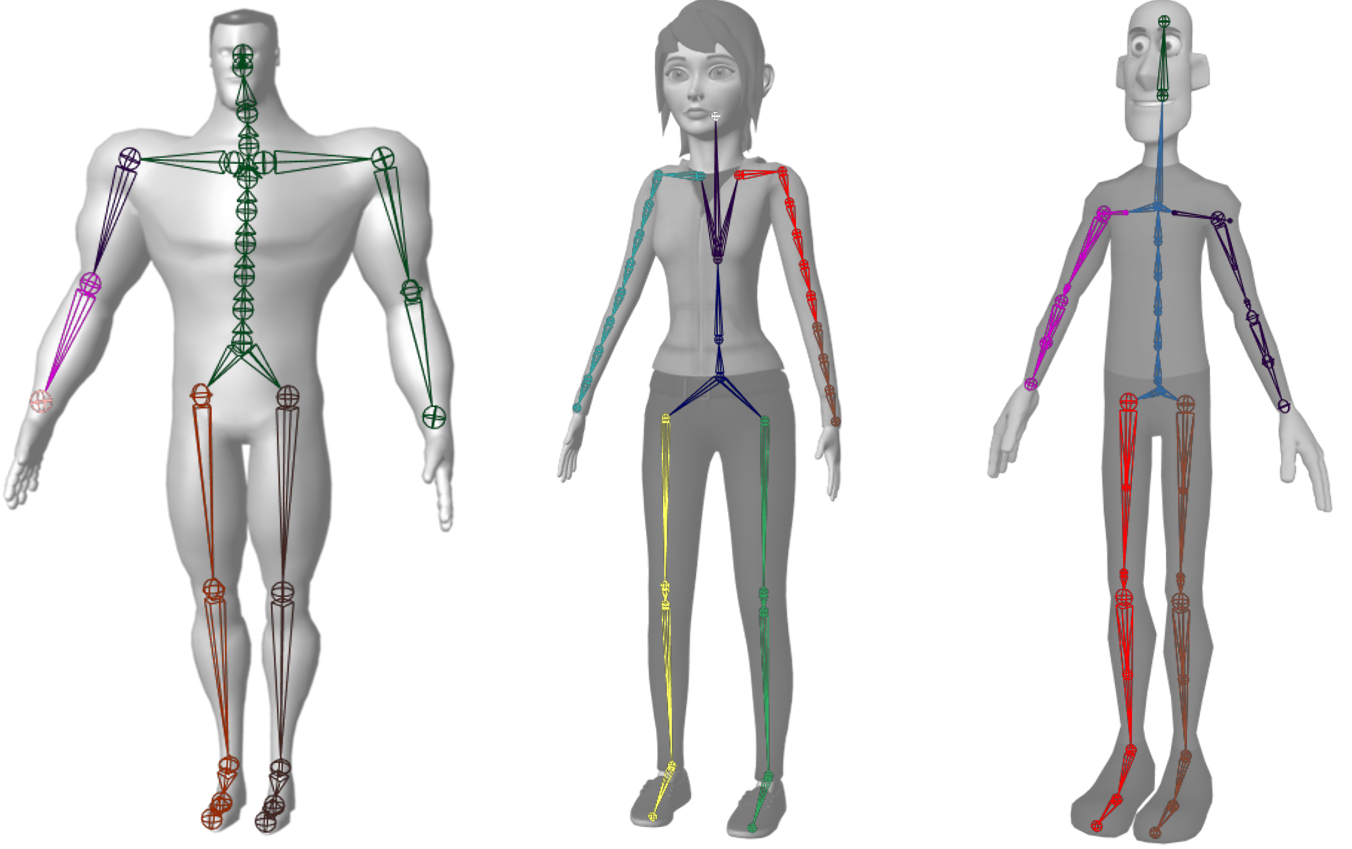
\includegraphics[width=0.85\linewidth]{images/bodyPartGrouping}
  \caption{Snapshots of various rig  grouping results}
  \label{fig:rigGroupingResult}
\end{figure}
Figure~\ref{fig:correlationMap}(right) shows an example of $G$. In our experimental results, we found that each $g_i$ is similar to the body part of a character, such as the limbs or the spine(Figure~\ref{fig:rigGroupingResult}). As our rig analysis process divides a complex non-linear full body problem into mutually independent body part sub-problems, our optimization can be performed close to linear relationship between the rig space and the skeleton space. 

